\section{IR with Mixed Precision}
\label{sec:mixed_precision}

As a direct consequence of the relation between working precision and condition number of the matrix $A$ (see Table~\hyperref[tab:ir_bounds]{\ref{tab:ir_bounds}} and the discussion in Chapter~\hyperref[chap:iterative_refinement]{\ref{chap:iterative_refinement}}), the convergence of LU-based iterative refinement is bound by the reciprocal of the working precision $u$. In the case of double precision ($u \approx 10^{-16}$), this translates to $\kappa_\infty(A) \leq 10^{16}$ as the maximum condition number for which convergence of the algorithm can be expected. This fact can be observed on the simple test case of a $100 \times 100$ matrix illustrated in Figure~\hyperref[fig:lue_ir]{\ref{fig:lue_ir}}.

\begin{figure}[h]
\centering
\begin{subfigure}{.5\textwidth}
  \centering
  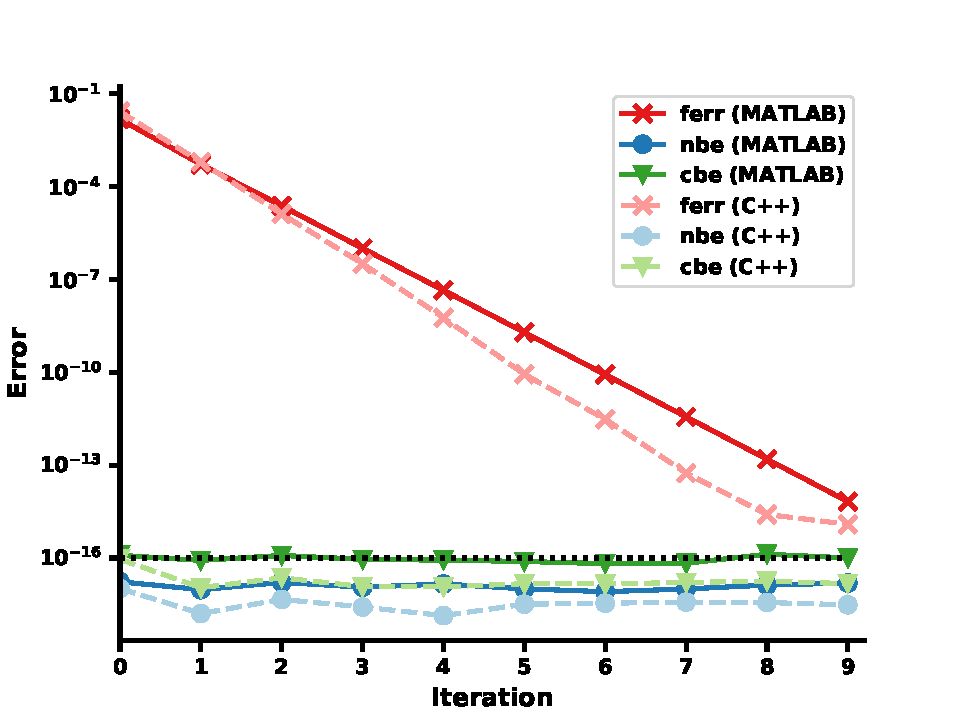
\includegraphics[width=\linewidth]{chapters/5_experiments/figures/LUe16.pdf}
  \caption{Convergence for $\kappa_\infty(A) = 10^{16}$}
  \label{fig:lue16}
\end{subfigure}%
\begin{subfigure}{.5\textwidth}
  \centering
  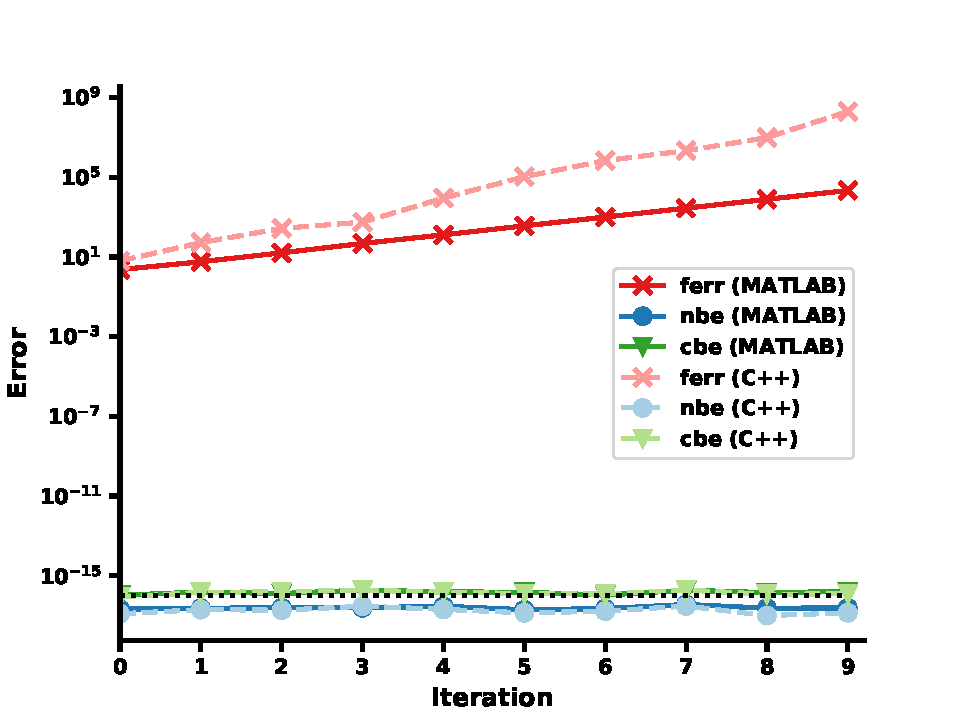
\includegraphics[width=\linewidth]{chapters/5_experiments/figures/LUe18.pdf}
  \caption{Divergence for $\kappa_\infty(A) = 10^{18}$}
  \label{fig:lue18}
\end{subfigure}
\caption[LU-based IR]{Convergence behaviour of LU-based iterative refinement for different condition numbers. Comparison between the MATLAB implementation from \cite{carson_new_2017} and the new C++ code (ferr = forward error, nbe = norm-wise backward error, cbe = component-wise backward error).}
\label{fig:lue_ir}
\end{figure}

The matrix was created using the build-in MATLAB function \textit{gallery('randsvd',kappa, mode)}, where \textit{kappa} specifies the 2-norm condition number and the parameter \textit{mode} refers to the distribution of the singular values (in this case $mode=2$ was used). The plots show the behaviour of the forward error ($ferr$, in red), norm-wise relative backward error ($nbe$ in blue) and component-wise relative backward error ($cbe$ in green). The dotted black line indicates the accuracy of the working precision $u$. The plots show the convergence behaviour of iterative refinement for very ill-conditioned matrices ($\kappa_\infty(A)=10^{16}$ and $\kappa_\infty(A)=10^{18}$). The solver is LU factorization computed in the working precision (double), while the residuals are accumulated in quadruple precision.

As expected from such high condition numbers, the forward error of the initial solution is quite large and close to $1$, while both backward errors remain small. If the condition number remains within the upper bound previously mentioned, iterative refinement is able to reduce the error in each iteration, converging to a solution (almost) accurate to precision $u$. This behaviour is depicted in Figure~\hyperref[fig:lue16]{\ref{fig:lue16}}. When the condition number becomes too large however, the solution starts to diverge and LU-based IR is no longer beneficial, as is shown in the case of Figure~\hyperref[fig:lue18]{\ref{fig:lue18}} (note that a condition number of $10^{18}$ has been chosen for clarity, $10^{17}$ would be sufficient to evoke this behaviour).

In order to obtain accurate results even for very ill-conditioned systems, \cite{carson_new_2017} introduced GMRES-based iterative refinement. In this approach, the LU factors are only used as a preconditioner to a modified GMRES variant, enabling the correction equation to be solved at a higher accuracy. Doing this removes the direct dependency on the precision of the LU factors, which consequently relaxes the constraint on the condition number. The convergence behaviour for this algorithm (on the same test matrices) is given in Figure~\hyperref[fig:gmrese_ir]{\ref{fig:gmrese_ir}}.

\begin{figure}[h]
\centering
\begin{subfigure}{.5\textwidth}
  \centering
  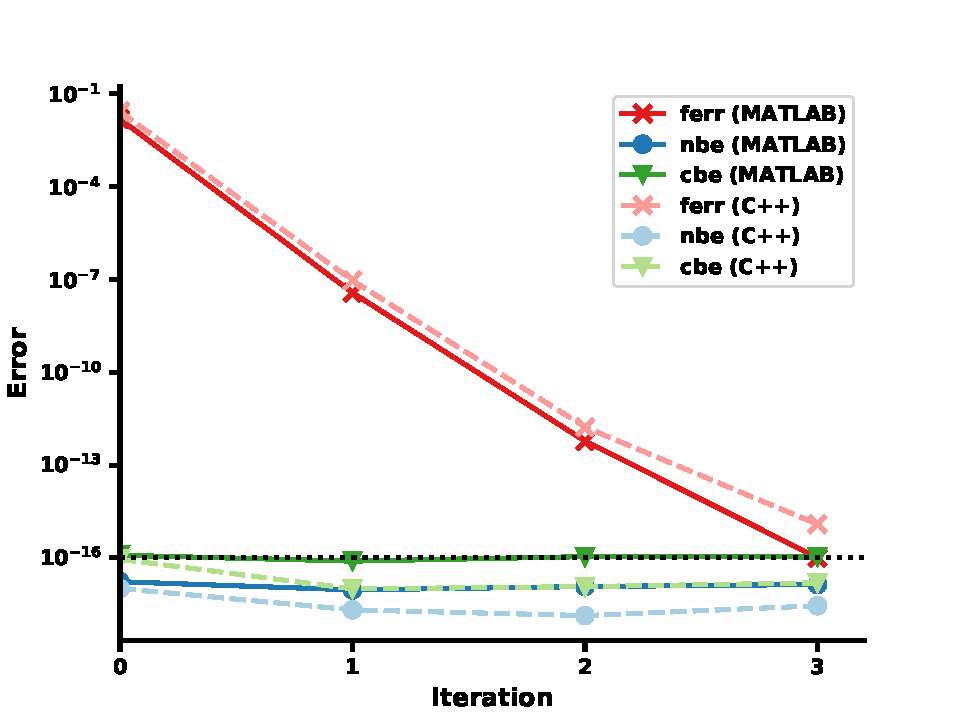
\includegraphics[width=\linewidth]{chapters/5_experiments/figures/GMRESe16.pdf}
  \caption{Convergence for $\kappa_\infty(A) = 10^{16}$}
  \label{fig:gmrese16}
\end{subfigure}%
\begin{subfigure}{.5\textwidth}
  \centering
  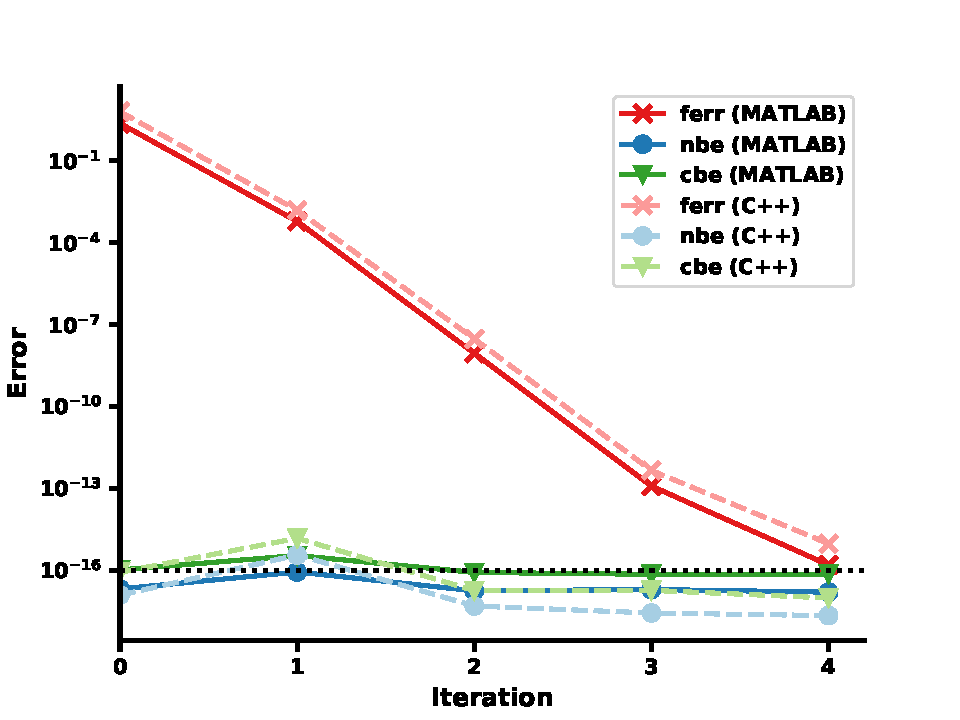
\includegraphics[width=\linewidth]{chapters/5_experiments/figures/GMRESe18.pdf}
  \caption{Convergence for $\kappa_\infty(A) = 10^{18}$}
  \label{fig:gmrese18}
\end{subfigure}
\caption[GMRES-based IR]{Convergence behaviour of GMRES-based iterative refinement for different condition numbers. Comparison between the MATLAB implementation from \cite{carson_new_2017} and the new C++ code (ferr = forward error, nbe = norm-wise backward error, cbe = component-wise backward error).}
\label{fig:gmrese_ir}
\end{figure}

There are two important observations to be made. First, as can be seen from Figure~\hyperref[fig:gmrese18]{\ref{fig:gmrese18}}, the algorithm converges to a solution accurate to working precision (i.e. double) even if $\kappa_\infty(A) > 10^{16}$. Therefore, this approach is promising for very ill-conditioned systems, even though the boundaries for convergence remain (currently) unclear (see \cite{carson_new_2017}). However, it has been demonstrated by \cite{carson_accelerating_2018}, that this method is able to tolerate LU factors that are computed at half the working precision. 

Secondly, as revealed by a comparison of Figure~\hyperref[fig:lue_ir]{\ref{fig:lue_ir}} \& \hyperref[fig:gmrese_ir]{\ref{fig:gmrese_ir}}, the necessary number of iterative refinement steps is reduced when compared to the LU-based algorithm. Despite a lower number of steps, the GMRES-based variant generally takes longer to execute, because the true cost is hidden within the GMRES iterations. When the convergence tolerance of GMRES is set to $10^{-4}$ (as proposed in \cite{carson_new_2017}), the average number of GMRES iterations for the above test matrices is $16$ for each IR step. Consequently, performance is highly dependent on the convergence of GMRES and thus on the distribution of the singular values. Hence, for most practical use-cases, the increased numerical stability is associated with a higher runtime and unless the system is very ill-conditioned, standard LU-based iterative refinement is usually the preferable choice.

Nonetheless, due to its tolerance for low-precision LU factors, the method might still be beneficial for general systems, if the iterative refinement process is generalized to three precisions. In this case, the reduced cost of the factorization might be enough to offset the additional iterations, resulting in a better performance overall. Since traditional iterative refinement is directly dependent on the accuracy of the factorization, its usefulness for low-precision calculations is limited as well. The examples provided in Figure~\hyperref[fig:lu_ir3]{\ref{fig:lu_ir3}} demonstrate the breakdown of IR for a condition number of $\kappa_\infty (A)=10^9$, if the factorization is calculated in single precision. In such a case does not decrease at all, no matter how many iterations are executed.
It is noteworthy, that this restriction is independent of how the other precisions are chosen and cannot be offset by, for example, calculating the residuals in twice the working precision.

\begin{figure}[h]
\centering
\begin{subfigure}{.5\textwidth}
  \centering
  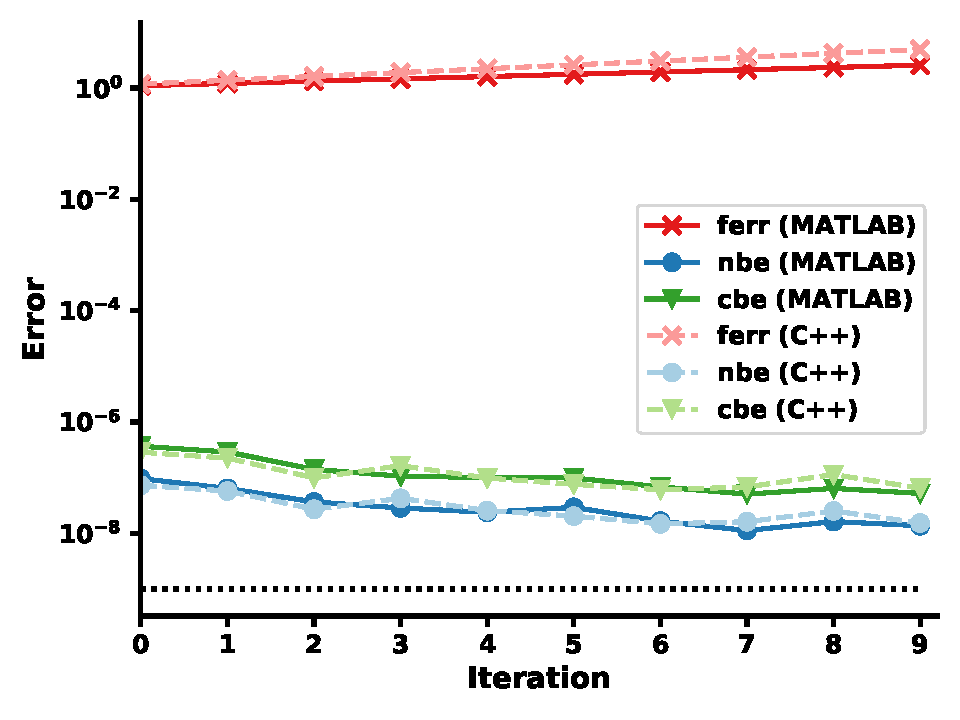
\includegraphics[width=\linewidth]{chapters/5_experiments/figures/LUsdd.pdf}
  \caption{LU-IR (single - double - double)}
  \label{fig:lusdd}
\end{subfigure}%
\begin{subfigure}{.5\textwidth}
  \centering
  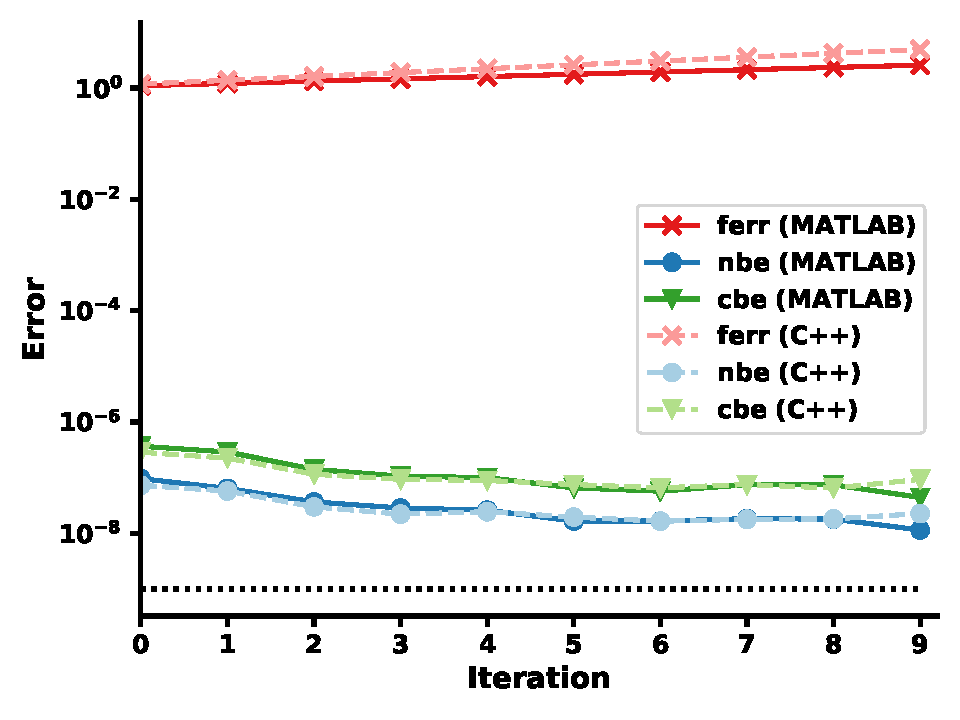
\includegraphics[width=\linewidth]{chapters/5_experiments/figures/LUsdq.pdf}
  \caption{LU-IR (single - double - quadruple)}
  \label{fig:lusdq}
\end{subfigure}
\caption[LU-based IR (single precision factorization)]{Convergence behaviour of LU-based iterative refinement for a condition number of $\kappa_\infty (A)=10^9$, when the LU factors are calculated in single precision. Comparison between the MATLAB implementation from \cite{carson_new_2017} and the new C++ code (ferr = forward error, nbe = norm-wise backward error, cbe = component-wise backward error).}
\label{fig:lu_ir3}
\end{figure}

GMRES-based iterative refinement, on the other hand, is able to achieve a solution accurate to working precision, even if only single precision LU factors are available. As can be observed in Figure~\hyperref[fig:gmres_ir3]{\ref{fig:gmres_ir3}}, the accuracy of the obtained solution by GMRES-IR in 3 precisions is equivalent to traditional iterative refinement in double precision. The results in Figure~\hyperref[fig:gmressdq]{\ref{fig:gmressdq}} were obtained by using a tolerance of $10^{-6}$ for the GMRES part of the algorithm, which converged after $2-3$ in each IR step. Hence, the actual performance overhead should not be too large and this variant might be beneficial on systems where fast single precision arithmetic is available.

\begin{figure}[h]
\centering
\begin{subfigure}{.5\textwidth}
  \centering
  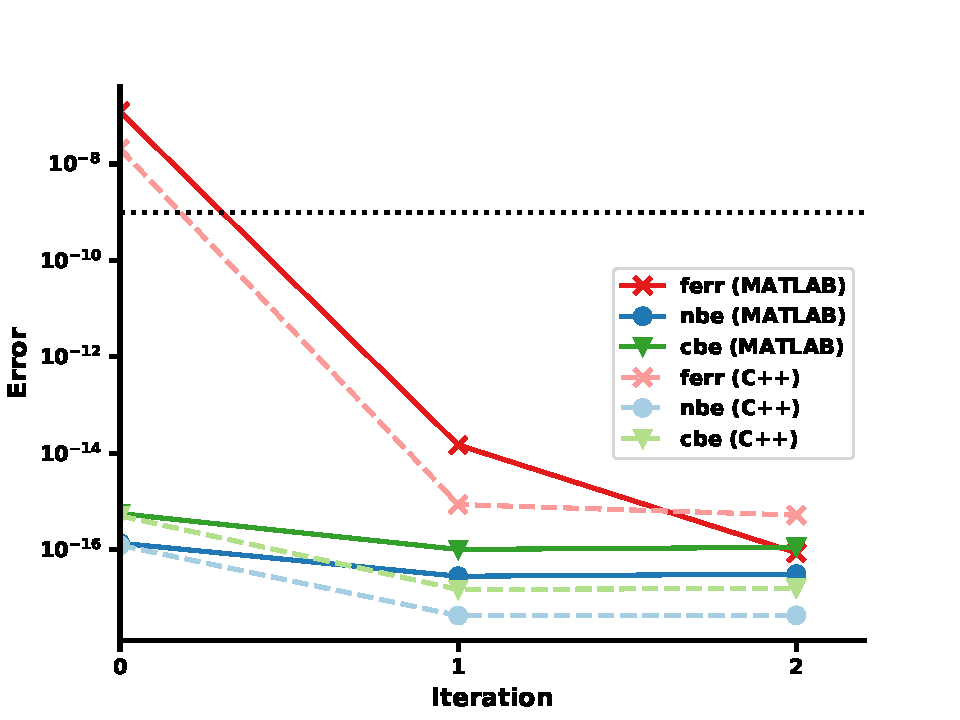
\includegraphics[width=\linewidth]{chapters/5_experiments/figures/LUddq.pdf}
  \caption{LU-IR (double - double - quadruple)}
  \label{fig:luddq}
\end{subfigure}%
\begin{subfigure}{.5\textwidth}
  \centering
  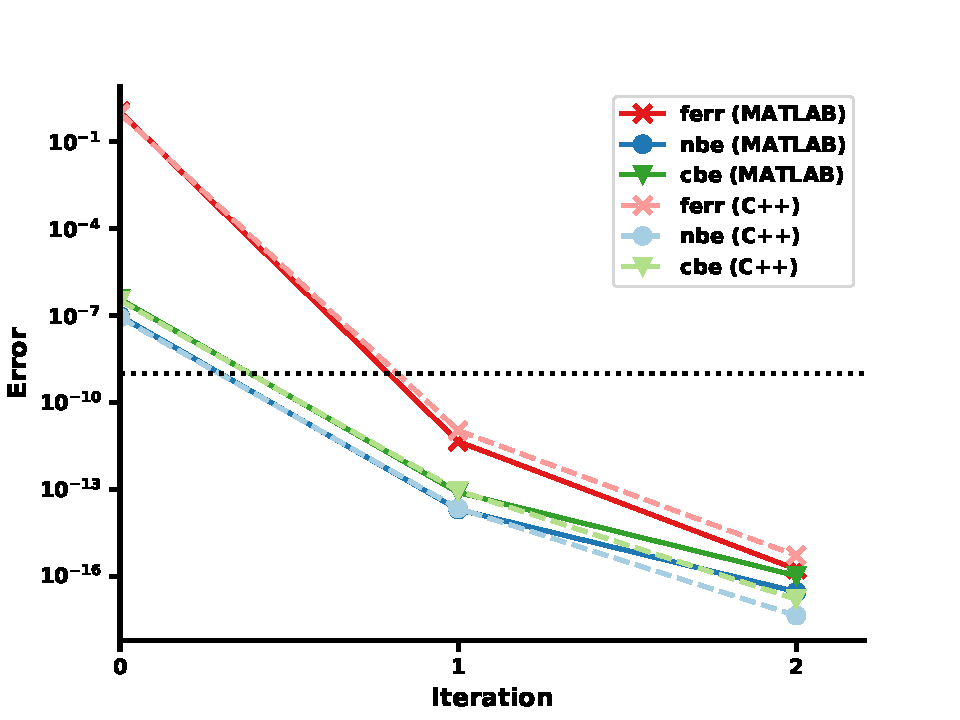
\includegraphics[width=\linewidth]{chapters/5_experiments/figures/GMRESsdq.pdf}
  \caption{GMRES-IR (single - double - quadruple)}
  \label{fig:gmressdq}
\end{subfigure}
\caption[GMRES based IR in 3 Precisions]{Convergence behaviour of GMRES-based iterative refinement for a condition number of $\kappa_\infty (A)=10^9$, when the LU factors are calculated in single precision in contrast to LU-based double precision IR. Comparison between the MATLAB implementation from \cite{carson_new_2017} and the new C++ code (ferr = forward error, nbe = norm-wise backward error, cbe = component-wise backward error).}
\label{fig:gmres_ir3}
\end{figure}

For iterative refinement in two precisions (single and double), \cite{langou_exploiting_2006} demonstrated that on certain microprocessor architectures, a speed-up of up to $4.7$ can be observed when compared to a direct solver in double precision. This routine is available as a LAPACK function under the name \textit{DSGESV}, being equivalent to LU-based iterative refinement with precisions single - double - double. However, for iterative refinement in three precisions, similar performance analyses are not yet available. Therefore, the following methods are compared with regards to their performance on different linear systems:
\begin{itemize}
    \item \textit{DGESV}: in double precision (LAPACK routine that solves a linear system directly via LU factorization)
    \item \textit{DSGESV}: single - double - double precision (LAPACK routine based on iterative refinement of a single precision LU factorization)
    \item \textit{LU-IR (sdd)}: single - double - double precision (same as DDGESV but implemented in this research)
    \item \textit{LU-IR (ddq)}: double - double - quadruple precision (LU-based IR with double precision factorization, implemented in this research)
    \item \textit{GMRES-IR (sdq)}: single - double - quadruple precision (GMRES based IR with single precision factorization, implemented in this research)
\end{itemize}

\noindent But before going into details about the execution time, it is important to confirm the error bound of the different algorithms. For this purpose, a $512 \times 512$ matrix is used created via the \textit{gallery} function using $mode = 1$ (i.e. one large singular value). Since both backward errors stay safely below the working precision (i.e. $\leq 10^{-16}$) if convergence is achieved, this analysis will be focused mainly on the forward error. The results obtained for this comparison are illustrated in Figure~\hyperref[fig:ir3_ac]{\ref{fig:ir3_ac}}. A few remarks have to be made with regards to the interpretation of those experiments. First, all measurements below $\leq 10^{-20}$ have been clipped to the same value to maintain readability of the figure. Second, the errors achieved by \textit{DSGESV} and \textit{LU-IR (sdd)} are almost identical and the latter has been therefore omitted. Third, if it does not converge within 30 iterations \textit{DSGESV} falls back to the \textit{DGESV} routine in double precision making the results identical. Therefore, no error is reported if \textit{DSGESV} fails to achieve convergence.

\begin{figure}[h]
    \centering
    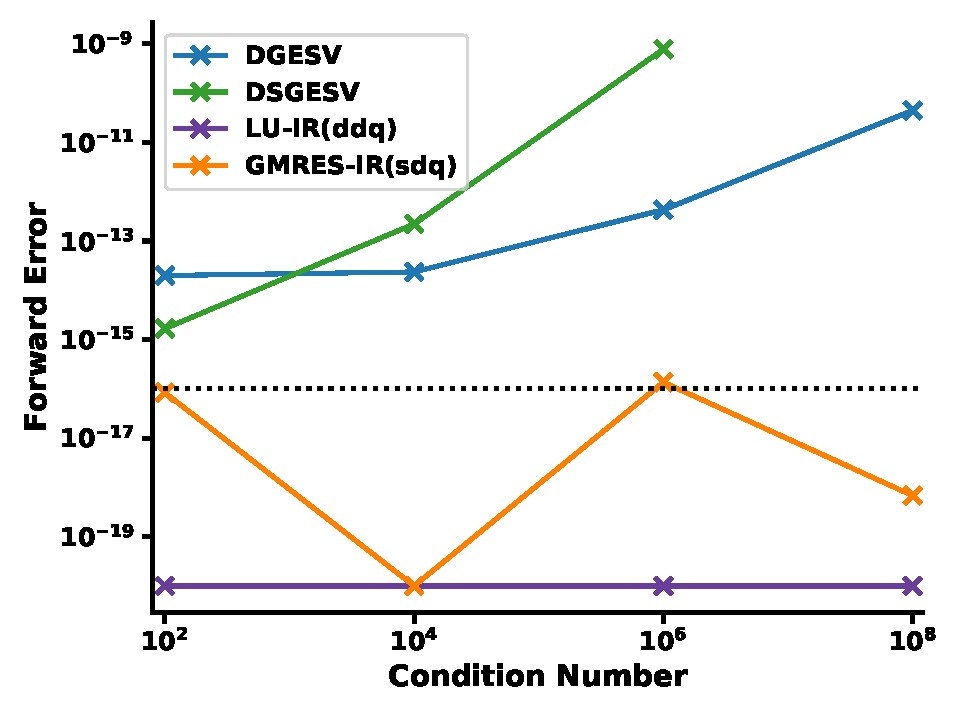
\includegraphics[width=0.7\linewidth]{chapters/5_experiments/figures/IR3_acc.pdf}
    \caption[IR - Forward Error 1]{Forward error analysis of different routines for solving a linear system. Note that DSGESV does not converge for $\kappa_\infty(A)=10^8$.}
    \label{fig:ir3_ac}
\end{figure}

Generally, it can be observed that the forward error of a direct solving approach (\textit{DGESV}) increases with the condition number of $A$. However, up to a condition number of $u^{-1}$, this can be countered by using a few iterative refinement steps to obtain a solution accurate to working precision (\textit{LU-IR (ddq)}). If the factorization is computed in single precision (\textit{DSGESV} and \textit{GMRES-IR (sdq)}), traditional LU-based iterative refinement fails as the condition number approaches the reciprocal of the factorization precision (i.e. $\approx 10^8$) and both the error as well as the number of iterations increases with the condition number. In contrast, GMRES-based IR is able to maintain a solution accurate to working precision, even if $A$ becomes increasingly ill-conditioned.

It is worth mentioning that the the achieved accuracy can be guaranteed independent of the matrix size $n$. As shown in Figure~\hyperref[fig:ir3_n]{\ref{fig:ir3_n}}, the error remains relatively constant for the different routines, depending solely on the condition number of $A$. Most interestingly, the number of iterative refinement steps necessary follows a similar trend, remaining constant with regards to the matrix size. A similar observation can be made for the number of GMRES iterations, even if the variation is slightly larger in this case.

\begin{figure}[h]
    \centering
    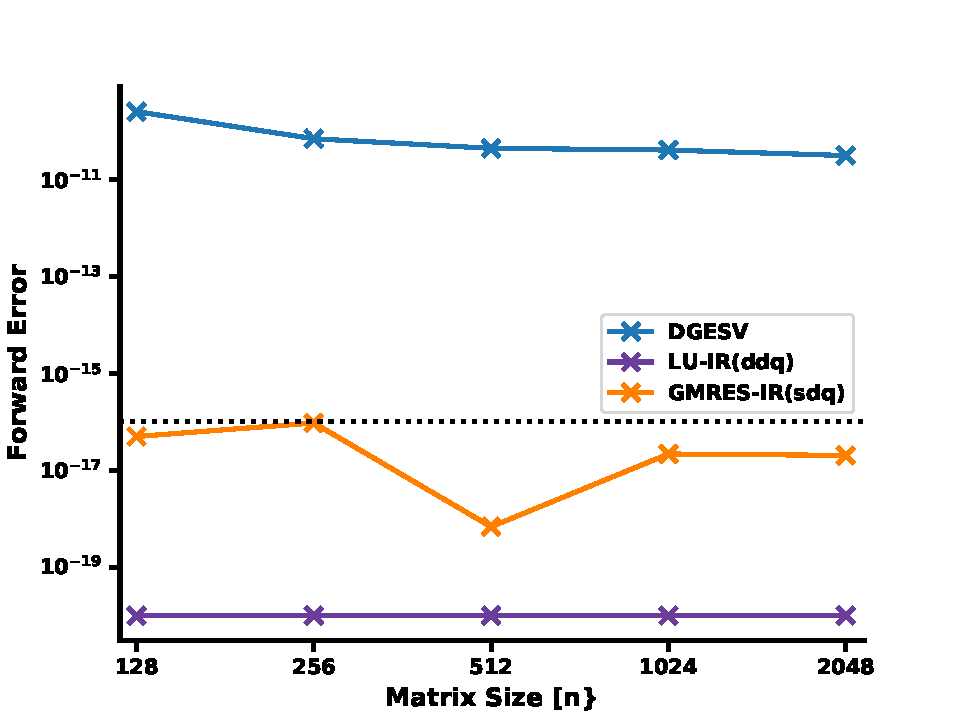
\includegraphics[width=0.7\linewidth]{chapters/5_experiments/figures/IR3_n.pdf}
    \caption[IR - Forward Error 2]{Forward error analysis with respect to the matrix size $n$ for $\kappa_\infty(A)=10^8$. The accuracy remains relatively constant.}
    \label{fig:ir3_n}
\end{figure}


\begin{figure}[h]
    \centering
    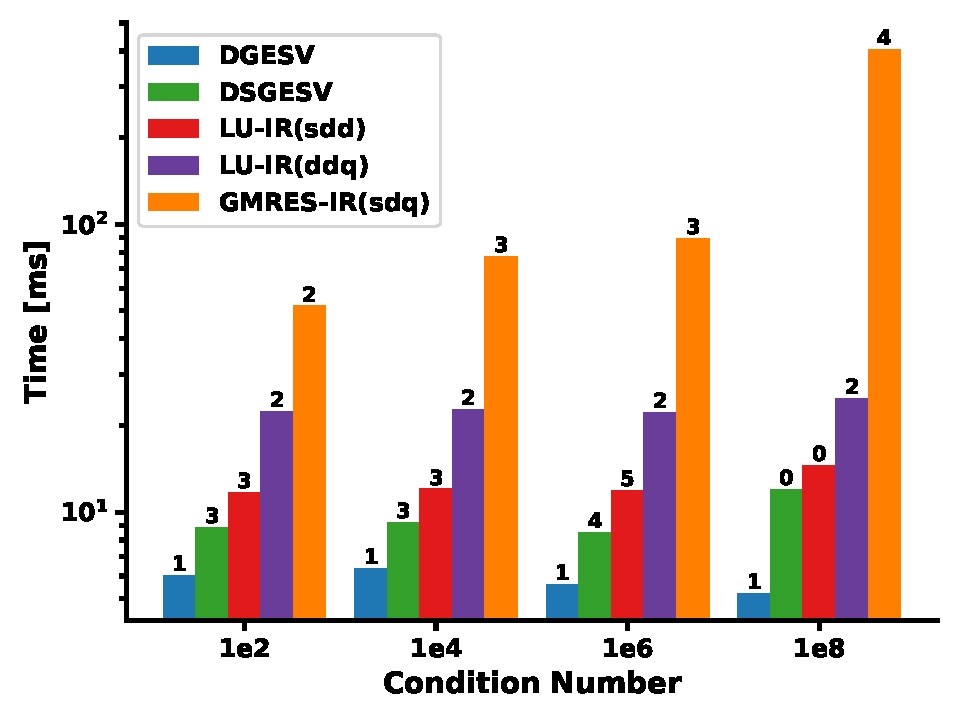
\includegraphics[width=0.7\linewidth]{chapters/5_experiments/figures/IR3_runtime.pdf}
    \caption[IR - Runtime]{Runtime analysis with respect to the condition number for a constant matrix size ($n=512$). The number of iterations for each method is annotated at the top of the bar and is equal to the number of created solutions. $0$ indicates that the routine did not converge.}
    \label{fig:ir3_time}
\end{figure}

Turning to the actual runtime behaviour, the elapsed real time (or wall-clock time) is measured for all routines. This represents the time that has passed between starting the solver and obtaining a solution accurate to working precision (or a failure signal in case of divergence). Each measurement has been performed five times, taking the mean as a representative for the computational time. The obtained measurements are displayed in Figure~\hyperref[fig:ir3_time]{\ref{fig:ir3_time}}. It needs to be remarked that there seems to be a large overhead for the first call to the LAPACK functions in each experiment, influencing the performance of those routines for $\kappa_\infty(A)=10^2$. Therefore, those measurements are not representative and cannot be interpreted easily. Since the matrix size does not change, the performance of \textit{DGESV} and \textit{LU-IR (ddq)} (always two iterations) should remain somewhat constant, because they are independent of the condition number. Furthermore, it is noticeable that the single precision factorization of the \textit{DSGESV} is advantageous, except for the ill-conditioned case where no convergence can be achieved (this is indicated by a $0$ on top of the bar, but in reality this routine computes 30 iterations and then falls back to \textit{DGESV}, explaining the large time to solution).

The results for \textit{LU-IR (sdd)} indicate the difference between a highly optimized two precision kernel and the three precision variant of the algorithm, usually requiring the same number of iterations. The performance of \textit{LU-IR (ddq)} shows that the overhead of calculating the residuals in quadruple precision is considerable, because this floating-point format is not directly supported in hardware. Finally the running time of \textit{GMRES-IR (sdq)} hinges on the number of internal GMRES iterations, which are quite costly due to the high-precision calculations involved. 

There are three main conclusions to be drawn from these results:
\begin{enumerate}
    \item The performance of iterative refinement depends on the condition number of the matrix, resulting in slow convergence or breakdown for ill-conditioned systems.
    \item The higher error bound of \textit{GMRES-IR (sdq)} comes at the cost of additional calculations and is only efficient for a low number of GMRES iterations.
    \item The cost of floating-point arithmetic that is not supported in hardware is considerable and better results might be expected from a half - single - double precision approach.
\end{enumerate}

\noindent Even though some of the solution techniques clearly perform better than others, they all share the same time complexity of $\mathcal{O}(n^3)$. This is illustrated in Figure~\hyperref[fig:ir3_scale]{\ref{fig:ir3_scale}} for the direct solving as well as LU- and GMRES-based iterative refinement. 

\begin{figure}[h]
    \centering
    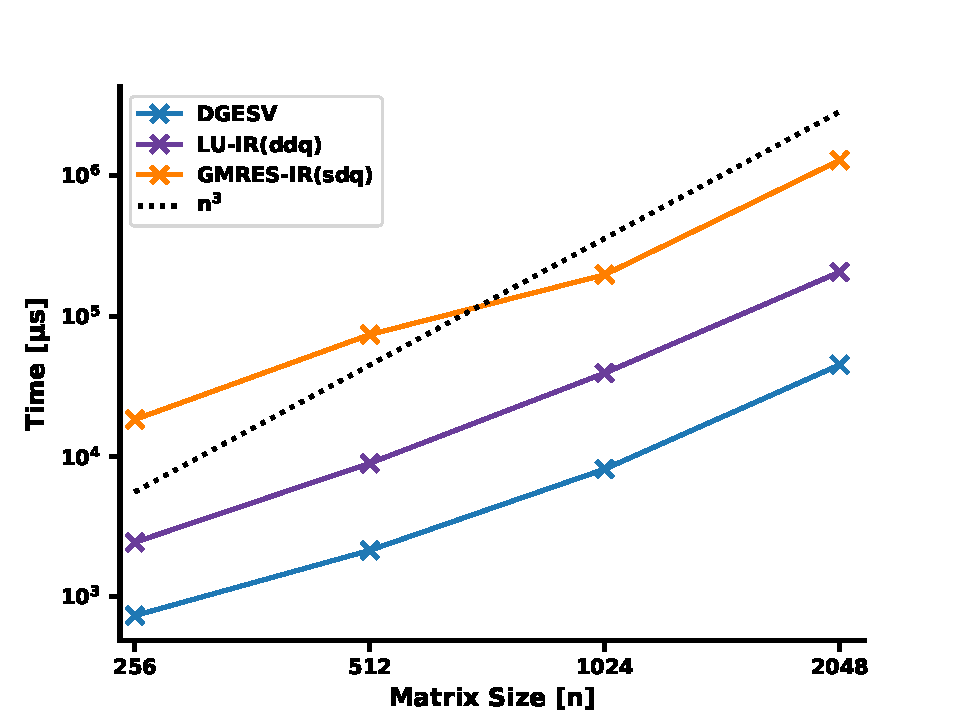
\includegraphics[width=0.7\linewidth]{chapters/5_experiments/figures/IR3_scaling.pdf}
    \caption[IR - Scaling]{Runtime analysis with respect to the matrix size for a constant condition number ($\kappa_\infty(A)=10^5$). All methods remain within $\mathcal{O}(n^3)$.}
    \label{fig:ir3_scale}
\end{figure}